%--------------------------------------------------------------------
% 3 Diseño – SEPA Request‑to‑Pay Prototype (Clase `article`)
%--------------------------------------------------------------------
\chapter{Diseño}
\label{sec:diseno}

En este apartado se detalla la estrategia adoptada para \emph{emular, con un prototipo funcional, el comportamiento extremo‑a‑extremo del servicio SEPA RTP}. Se parte de los requisitos funcionales publicados en el \emph{EPC RTP Rulebook 4.0} y se traducen a casos de uso concretos, modelo de datos y flujos de interacción que servirán de base a la implementación descrita en el apartado~\ref{sec:implementacion}. Se persigue, ante todo, una visión que facilite al lector identificar primero el~\emph{qué} resuelve la solución y, a continuación, el~\emph{cómo} se materializa.

\section{Objetivos técnicos}
\label{subsec:diseno_objetivos}


El diseño e implementación del prototipo desarrollado responden a los objetivos técnicos fundamentales definidos en el capítulo \ref{subsec:Objetivos}. Estos objetivos buscan demostrar que el esquema SEPA RTP puede superar las limitaciones del sistema tradicional de domiciliación bancaria, ofreciendo una solución moderna, eficiente y adaptada a las demandas de la economía digital actual. A continuación se detallan estos objetivos en orden de prioridad, explicando qué se pretende conseguir con cada uno, cómo se implementaría y por qué son esenciales para el éxito del prototipo.

\begin{enumerate}[label=\textbf{\arabic*}]
  % Objetivo 1
  \item \textbf{Reproducir el ciclo RTP extremo a extremo}
    
    El propósito fundamental del prototipo es desarrollar un sistema que emule de manera completa y fiel el ciclo del esquema RTP, abarcando todas las etapas definidas en la tabla de pasos del SRTP \ref{tab:srtp-steps-b}. Esto implica que el prototipo debe ser capaz de replicar el flujo completo del proceso, desde el momento en que el beneficiario inicia una solicitud de pago hasta la resolución final por parte del pagador, incluyendo tanto escenarios exitosos como aquellos en los que se producen errores o rechazos.
    
    Se quiere que el sistema emule todas las operaciones clave del RTP: la creación de la solicitud por parte del beneficiario, la validación por parte de los PSP y la decisión final del pagador. Esto incluye manejar situaciones reales, como la falta de fondos del pagador o errores en los datos de la solicitud, para garantizar que el prototipo sea robusto y represente fielmente cómo funcionaría un proveedor de RTP en un entorno real.
    
    El sistema implementará una API basada en HTTP/JSON que cubra las operaciones principales de RTP. Además se diseñarán mecanismos para simular errores como IBAN inválidos o saldos insuficientes, y se registrarán los resultados de cada etapa para analizar su comportamiento.
    
    Reproducir el ciclo completo es esencial para demostrar que el RTP puede ser una alternativa viable al SDD, resolviendo los problemas como la lentitud o la falta de interacción en tiempo real y proporcionando una base sólida para futuras implementaciones reales.

  % Objetivo 2
  \item \textbf{Ofrecer notificación en tiempo real}
    
    Dado que el RTP es un esquema diseñado para operar en un entorno digital y online, se busca garantizar que todas las partes involucradas reciban información inmediata sobre cualquier cambio o evento relacionado con la solicitud de pago.

   Se quiere que el sistema notifique instantáneamente a los actores cada vez que ocurra un evento significativo, como la creación de una solicitud RTP, su validación por un PSP o la decisión final del pagador. Esto simulará la experiencia que un usuario tendría al recibir una notificación en su aplicación bancaria, permitiendo al pagador reaccionar rápidamente y al beneficiario conocer el estado de su solicitud sin demoras.

    Se utilizarán eventos de WebSocket, una tecnología que permite una comunicación bidireccional en tiempo real entre el servidor y los clientes. Por ejemplo, cuando el beneficiario crea una solicitud, el sistema enviará una notificación al pagador a través de una sala específica WebSocket; de manera similar, cuando el pagador tome una decisión, el beneficiario será informado de inmediato. Este enfoque asegura que las actualizaciones sean push en lugar de depender de consultas manuales.

    La inmediatez es una de las principales ventajas de RTP frente a SDD, que opera en un modelo offline con retrasos de días. Este objetivo refleja la necesidad de una experiencia de usuario fluida y ágil, alineada con las expectativas actuales de rapidez en el comercio digital.
  
  % Objetivo 3
  \item \textbf{Garantizar seguridad y trazabilidad}

    La seguridad y la capacidad de rastrear todas las acciones realizadas son pilares fundamentales para cualquier sistema de pagos, especialmente uno que aspire a ser adoptado en un contexto real.

    Se quiere que cada cambio de estado en una solicitud RTP quede registrado de forma segura e inalterable en la base de datos, permitiendo reconstruir el historial completo de cualquier solicitud en cualquier momento. Esto servirá para auditar el sistema, prevenir fraudes y resolver disputas entre las partes.

    Cada transición de estado se almacenará junto con un hash SHA-256, que asegura la integridad de los datos, y una marca de tiempo en formato UTC, que indica el momento exacto de la acción. Por ejemplo, si un PSP valida una solicitud, se generará un registro con estos elementos, y cualquier intento de modificar los datos será detectable gracias al hash. Además se implementarán controles de acceso por roles para limitar quién puede realizar cada acción.

    Sin seguridad y trazabilidad, el sistema será vulnerable a manipulaciones o ataques, lo que comprometería su credibilidad. Este objetivo asegura que el prototipo cumpla con los requisitos de confianza y auditoría, esenciales para su evolución hacia un sistema de producción.
  
  % Objetivo 4
  \item \textbf{Persistir la información de forma ligera}

    Es importante diseñar un sistema de almacenamiento que sea práctico para las fases iniciales del desarrollo y pruebas, pero que también permita crecer en el futuro si el prototipo se expande.

    Se quiere que la información generada por las solicitudes RTP se guarde de forma sencilla y sin requerir recursos excesivos durante el desarrollo, utilizando herramientas que no dependan de configuraciones complejas o servidores externos. Al mismo tiempo, quiero que el diseño sea flexible para adaptarse a necesidades mayores más adelante.

    Se empleará SQLite como base de datos, gestionada mediante SQLAlchemy, una biblioteca que facilita la interacción con los datos. SQLite es ideal para este prototipo porque es ligera, no requiere instalación adicional y funciona bien en entornos locales. Sin embargo, el sistema se estructurará de manera modular, permitiendo una migración futura a PostgreSQL u otra base de datos más robusta si el volumen de transacciones o usuarios aumenta.

    Un almacenamiento eficiente reduce la complejidad del desarrollo inicial y asegura que el prototipo sea fácil de instalar y probar. La flexibilidad para escalar es clave para que el sistema no quede obsoleto si se decide llevarlo a un entorno real.
  
  % Objetivo 5
  \item \textbf{Facilitar pruebas automatizadas e integración continua}

    Para garantizar la calidad y fiabilidad del prototipo, este objetivo busca establecer un proceso de verificación continua que detecte errores y asegure que el sistema funciona correctamente a medida que evoluciona.

    Se quiere crear un conjunto de pruebas que revisen automáticamente las funcionalidades del servidor y que estas pruebas se ejecuten de manera recurrente cada vez que se realicen cambios en el código. Esto asegurará que el sistema permanezca estable y funcional durante todo el desarrollo.

    Se diseñarán pruebas automáticas utilizando Postman, una herramienta que permite simular peticiones HTTP y validar las respuestas de la API. Estas pruebas cubrirán los endpoints principales y se integrarán en un flujo de integración continua.

    Las pruebas automatizadas son esenciales para mantener la calidad del software, especialmente en un prototipo que simula un sistema crítico como el RTP. Este objetivo reduce el riesgo de errores no detectados y facilita la incorporación de nuevas funcionalidades sin comprometer la estabilidad.

\end{enumerate}

\section{Actores y alcance}
\label{subsec:diseno_actores}

La emulacion del SRTP en este prototipo se basa en el modelo de cuatro esquinas expuesto anteriormente en la figura \ref{fig:4corner}. Este modelo es ampliamente utilizado en sistemas de pagos europeos porque proporciona un marco claro y seguro para gestionar transacciones, dividiendo las responsabilidades entre cuatro actores principales. Estos actores trabajan juntos para garantizar que una solicitud de pago fluya desde quien la inicia hasya quien debe responderla, pasando por intermediarios financieros que facilitan el proceso. A continuación se describen en detalle los actores y cómo interactúan, seguidos por una explicación del alcance de la emulación en el prototipo.

\textbf{Actores del modelo de cuatro esquinas}

Los cuatro actores que conforman el modelo son los siguientes:
\begin{description}
  \item[\textbf{Beneficiario.}]
  Es el comercio, empresa o persona que indica la solicitud de pago (RTP). Este actor es quien tiene la necesidad de recibir un pago, como un comercio enviando una factura a un cliente, una empresa de servicios solicitando el pago de una cuenta o incluso un individuo pidiendo dinero a otr. En el prototipo, el beneficiario es simulado para dar comienzo al proceso, enviando la solicitud de pago a su proveedor de servicios para que sea procesada.
  \item[\textbf{PSP Beneficiario.}]
  Este es el PSP que da soporte al beneficiario. Un PSP es tipicamente un banco, una entidad financiera o una plataforma de pagos que actúa en nombre del beneficiario. Su rol principal consiste en recibir la solicitud de pago iniciada por el beneficiario, verificar que sea válida y luego enrutarla hacia el PSP del pagador. En el prototipo, este actor simula esta función de validación y enrutamiento, asegurando que la solicitud avance al siguiente paso.
  \item[\textbf{PSP Pagador.}]
  Es el PSP que atiende al pagador final. Recibe la solicitud de pago enviada por el PSP beneficiario, la valida y la comunica al pagador para que tome una decisión. En un sistema real, si el pagador acepta la solicitud, el PSP pagador también ejecutaría la transferencia de fondos, pero en este prorotipo, como se detalla más adelante, esta parte no está incluida. Aquí, el PSp pagador simula la entrega de la solicitud y la recepción de la respuesta del pagador.
  \item[\textbf{Pagador.}]
  Es el cliente bancario o usuario final que recibe la solicitud de pago y decide si la acepta o la rechaza. En la vida real, esto podría ser una persona que recibe una notificación en su banca en línea o aplicación móvil, donde se le pide autorizar un pago. En el prototipo, el pagador es simulado para cerrar el ciclo de la solicitud, tomando la decisión final de aceptación o rechazo.
\end{description}

Estas interacciones entre los actores de ilustran en la figura \ref{fig:4corner}.

\paragraph{Alcance de la emulación.}  

El prototipo tiene como objetivo simular el flujo del esquema SRTP en un entorno controlado, pero con un alcance limitado para enfocarse en los aspectos esenciales del proceso de solicitud de pago. Esto significa que no replica todas las funcionalidades de un sistema RTP real, sino que prioriza ciertas partes para cumplir con los objetivos del proyecto. A continuación, se explica qué incluye la emulación, qué se deja fuera y las razones detrás de estas decisiones.

\begin{description}
  %\item[\textbf{Entorno de despliegue.}]
  %El prototipo opera en una red local utilizando \textit{Docker Compose}, una herramienta que permite gestionar varios contenedores Docker. En este caso, se crean cuatro contenedores, uno por cada actor, ejecutados sobre un sistema operativo Linux como host. Este enfoque simula un entorno distribuido donde cada actor opera de manera independiente, reflejando como funcionaría el esquema RTP en la realidad, pero dentro de un entorno aislado y fácil de configurar. Usar Docker Compose facilita la portabilidad y la reproducibilidad del prototipo, lo que es ideal para pruebas y demostraciones.
  \item[\textbf{Registro en la OSM.}]
  En un sistema RTP real, los actores deben estar registrados y autenticados a través de la OSM, una entidad central que asegura que todas las partes sean legítimas y cumplan con las reglas del esquema. Sin embargo, en este prototipo, no se aplica el registro en la OSM. En lugar de implementar este proceso, se asume que los actores ya están registrados y autenticados de antemano. Esta simplificación elimina la necesidad de desarrollar una lógica compleja de registro y autenticación, lo que reduce el esfuerzo de desarrollo y permite centrarse en el flujo de la solicitud de pago. Sin embargo, esto implica que el prototipo no abroda aspectos de seguridad relacionados con la verificación de identidad de los actores, una limitación aceptable para los fines de esta simulación.
  \item[\textbf{Materialización de la orden de pago SCT Inst.}]
  En un sistema RTP completo, cuando el pagador acepta la solicitud del pago, se genera una orden de pago mediante SEPA Inst, un esquema que permite transferenciuas de fondos instantáneas entre cuentas bancarias en la zona SEPA. En este prototipo, no se materializa la órden de pago SCT Inst después de que la solicitud es aceptada. Esto significa que el sistema simula todo el proceso hasta la aceptación o rechazo de la solicitud, pero no ejecuta la transferencia de dinero real. Esta decisión se basa en las limitaciones discutidas en el SRTP Scheme Rulebook \cite{epc014}, y se justifica porque el objetivo principal del prototipo es demostrar la interacción entre los actores y la lógica de la solicitud de pago, no integrar un sistema de pagos real. Incluir la ejecución de SCT Inst requeriría conectar el prototipo a servicios bancarios o simular un sistema financiero completo, lo que añadiría una complejidad innecesaria a este proyecto.
\end{description}

En resumen, la emulación sigue el modelo de cuatro esquinas de la EPC, con cuatro actores claramente definidos que interactúan en una red local. El prototipo se centra en simular la solicitud de pago y las respuestas entre los actores, omitiendo deliberadamente el registro en la OSM y la materialización de la orden de pago SCT Inst para mantener el enfoque en los aspectos clave del RTP, alineándose con los objetivos del proyecto y las limitaciones establecidas.
\section{Requisitos}
\label{subsec:diseno_requisitos}

\subsection{Requisitos funcionales (RF)}
Los requisitos funcionales detallan las operaciones específicas que el sistema debe realizar para emular el esquema SRTP. Estos requisitos aseguran que el prototipo implementado cubra el flujo completo de una solicitud de pago, desde su creación hasta la decisión final, incluyendo las interacciones entre los actores del modelo de cuatro esquinas.

\begin{longtable}{@{}>{\raggedright\arraybackslash}p{0.11\textwidth}p{0.8\textwidth}@{}}
\toprule
\textbf{Id.} & \textbf{Descripción} \\
\midrule\endhead
RF-01 & El Beneficiario debe poder crear una solicitud RTP indicando el IBAN del pagador, el importe en una moneda compatible con ISO 4217 (por ejemplo, euros) y un concepto descriptivo en formato UTF-8. La solicitud debe ser enviada al PSP Beneficiario para su procesamiento. \\
RF-02 & El PSP Beneficiario debe validar la sintaxis y el formato de la solicitud RTP recibida, asegurando que cumpla con los estándares del esquema (por ejemplo, IBAN válido, importe correcto). Una vez validada, debe enrutar la solicitud al PSP pagador correspondiente. \\
RF-03 & El PSP pagador debe aplicar reglas básicas de \textsc{KYC} (\emph{Know Your Customer}) y \textsc{AML} (\emph{Anti-Money Laundering}), como verificar que el pagador esté registrado y tenga capacidad para responder a la solicitud. Tras la validación, debe presentar la solicitud al pagador para que tome una decisión. \\
RF-04 & El pagador debe poder aprobar o rechazar la solicitud RTP con un tiempo máximo, simulando la inmediatez del esquema RTP. La decisión debe ser comunicada de vuelta al PSP pagador. \\
RF-05 & El Beneficiario debe recibir una notificación inmediata sobre la decisión del pagador (aceptación o rechazo) a través del sistema de notificaciones en tiempo real. \\
RF-06 & Cualquier parte involucrada debe poder emitir una solicitud de cancelación (\emph{cancellation request}) antes de que se tome la decisión final sobre la solicitud RTP. \\
\bottomrule
\caption{Requisitos funcionales}
\label{tab:RF}
\end{longtable}

\subsection{Requisitos no funcionales (RNF)}
Los requisitos no funcionales especifican las cualidades y restricciones del sistema que garantizan su rendimiento, seguridad y mantenibilidad. Estos requisitos aseguran que el prototipo sea eficiente y adecuado para simular un sistema de pagos en tiempo real, incluso en un entorno controlado.

\begin{longtable}{@{}>{\raggedright\arraybackslash}p{0.11\textwidth}p{0.8\textwidth}@{}}
\toprule
\textbf{Id.} & \textbf{Descripción} \\
\midrule\endhead
RNF-01 & El sistema debe incluir documentación detallada sobre su arquitectura, componentes y cómo desplegarlo, para facilitar su comprensión y mantenimiento. \\
RNF-02 & Toda la comunicación entre los actores debe estar cifrada. Además, cada transición de estado de la solicitud RTP debe registrarse con una huella digital SHA-256 para garantizar la integridad y trazabilidad. \\
RNF-03 & El prototipo debe depender exclusivamente de tecnologías portables como Python 3.12 para el backend y SQLite para la persistencia de datos, asegurando su ejecución en cualquier entorno compatible. \\
\bottomrule
\caption{Requisitos no funcionales}
\label{tab:RNF}
\end{longtable}

Los requisitos enlazan con la implememtación \ref{sec:implementacion} y con pruebas de validación incluidas en el apartado~\ref{sec:validacion}. Además, cada transición de estado se acompaña de un identificador único para facilitar el seguimiento en los logs.

\section{Casos de uso}
\label{subsec:diseno_casos_uso}

Los casos de uso describen las interacciones clave entre los actores y el sistema para cumplir con los requisitos funcionales del esquema. A continuación, se presentan dos casos de uso: CU-01 para la creación de una solicitud RTP y CU-02 para la decisión sobre dicha solicitud.

\subsection{CU-01 Crear solicitud RTP}
Este caso de uso describe cómo el \textit{Beneficiario} inicia una solicitud de pago (\textit{Request To Pay}, RTP) y cómo esta es procesada por el \textit{PSP Beneficiario} para su enrutamiento al \textit{PSP pagador}.
\begin{description}
  \item[Actor primario] ~ \textit{Beneficiario}
  \item[Flujo principal] ~
    \begin{enumerate}
      \item El \textit{Beneficiario} envía una solicitud HTTP \texttt{POST /rtp} con los datos requeridos: IBAN del pagador, importe y concepto.
      \item El \textit{PSP Beneficiario} valida la sintaxis y el formato de la solicitud.
      \item Si es válida, el \textit{PSP Beneficiario} enruta la solicitud al \textit{PSP pagador}.
      \item El sistema responde con \texttt{RTP creado con exito} y un identificador único (\textit{RTP-ID}).
    \end{enumerate}
  \item[Escenarios alternativos] ~
    \begin{itemize}
      \item Si el IBAN es inválido, el sistema devuelve \texttt{RTP no creado con éxito (IBAN inválido)}.
      % \item Si el \textit{PSP pagador} no está disponible, se devuelve \texttt{RTP no creado con éxito (Pagador no encontrado)}.
    \end{itemize}
  \item[Requisitos cubiertos] ~
    \begin{itemize}
      \item \textbf{RF-01:} Creación de la solicitud RTP por el \textit{Beneficiario}.
      \item \textbf{RF-02:} Validación y enrutamiento por el \textit{PSP Beneficiario}.
    \end{itemize}
\end{description}

\subsection{CU-02: Decidir solicitud RTP}
Este caso de uso detalla cómo el \textit{pagador} recibe la solicitud RTP a través del \textit{PSP pagador}, toma una decisión (\textit{accept} o \textit{reject}), y cómo esta decisión se notifica a los demás actores.
\begin{description}
  \item[Actor primario] ~ \textit{pagador}
  \item[Flujo principal] ~
    \begin{enumerate}
      \item El \textit{PSP pagador} presenta la solicitud RTP al \textit{pagador}.
      \item El \textit{pagador} selecciona \textit{accept} o \textit{reject} dentro del tiempo límite.
      \item El \textit{PSP pagador} registra la decisión y notifica a los demás actores mediante eventos.
    \end{enumerate}
  \item[Escenarios alternativos] ~
    \begin{itemize}
      \item Si el \textit{pagador} no responde a tiempo, la solicitud se rechaza automáticamente.
    \end{itemize}
  \item[Requisitos cubiertos] ~
    \begin{itemize}
      \item \textbf{RF-03:} Presentación de la solicitud al \textit{pagador} por el \textit{PSP pagador}.
      \item \textbf{RF-04:} Decisión del \textit{pagador} en un tiempo máximo.
      \item \textbf{RF-05:} Notificación de la decisión al \textit{Beneficiario}.
    \end{itemize}
\end{description}

Los flujos completos se ilustran en los diagramas de secuencia (Fig.~\ref{fig:seq_cu01} y Fig.~\ref{fig:seq_cu02}).

\begin{figure}[htbp]
  \centering
  % placeholder
  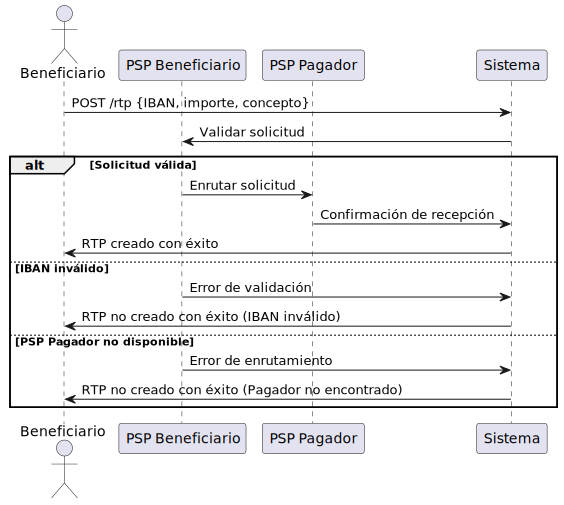
\includegraphics[width=.9\textwidth]{Imagenes/CU01.pdf}
  \caption{Diagrama de secuencia para CU‑01 (crear solicitud RTP).}
  \label{fig:seq_cu01}
\end{figure}

\begin{figure}[htbp]
  \centering
  % placeholder
  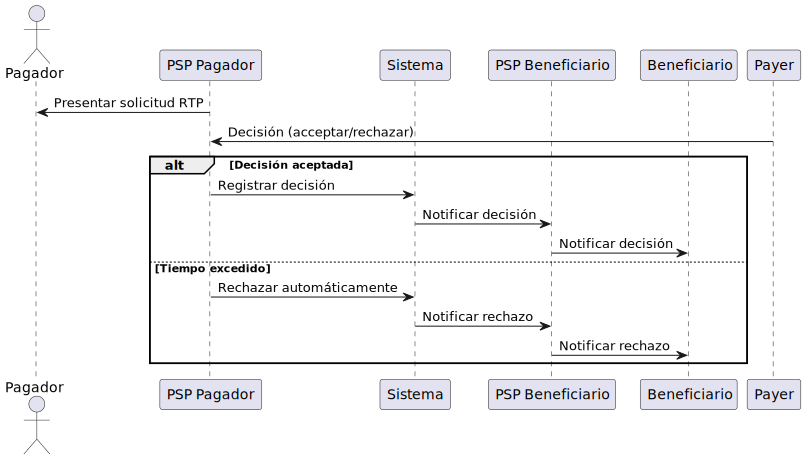
\includegraphics[width=.9\textwidth]{Imagenes/CU02.pdf}
  \caption{Diagrama de secuencia para CU‑02 (decisión final RTP).}
  \label{fig:seq_cu02}
\end{figure}

\section{Modelo de datos}
\label{subsec:diseno_datos}

% Descripción del esquema de la base de datos y referencia a la figura del modelo ER
El esquema de la base de datos, representado en el modelo entidad-relación (ER) de la Figura~\ref{fig:er_model}, está diseñado para soportar el flujo del esquema SRTP. Consta de tres tablas principales: \texttt{Actor}, \texttt{RTP} y \texttt{Log}, cada una con atributos específicos para almacenar la información necesaria del sistema.

% Inclusión de la figura del modelo ER
\begin{figure}[htbp]
  \centering
  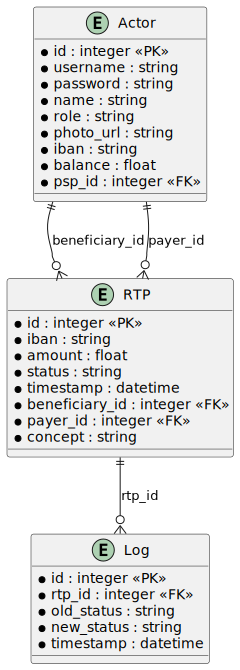
\includegraphics[width=0.9\textwidth, height=0.9\textheight, keepaspectratio]{Imagenes/ER.pdf}
  \caption{Modelo entidad-relación del prototipo.}
  \label{fig:er_model}
\end{figure}

% Listado de las tablas y sus atributos
Las tablas que componen el modelo de datos son las siguientes:

\begin{itemize}
  \item \textbf{Actor} (\texttt{id}, \texttt{username}, \texttt{password}, \texttt{name}, \texttt{role}, \texttt{photo\_url}, \texttt{iban}, \texttt{balance}, \texttt{psp\_id}) --- Almacena información sobre los actores involucrados en el sistema, como beneficiarios, pagadores y proveedores de servicios de pago (PSP). Sus atributos son:
    \begin{itemize}
      \item \texttt{id}: Identificador único del actor (clave primaria).
      \item \texttt{username}: Nombre de usuario único para autenticación.
      \item \texttt{password}: Contraseña del actor.
      \item \texttt{name}: Nombre completo del actor.
      \item \texttt{role}: Rol del actor, que puede ser \emph{beneficiary}, \emph{psp\_beneficiary}, \emph{psp\_payer} o \emph{payer}.
      \item \texttt{photo\_url}: URL o base64 de la foto del actor (opcional).
      \item \texttt{iban}: Número de cuenta bancaria internacional (IBAN).
      \item \texttt{balance}: Saldo disponible del actor.
      \item \texttt{psp\_id}: Referencia al actor que actúa como PSP (clave foránea a \texttt{Actor}).
    \end{itemize}

  \item \textbf{RTP} (\texttt{id}, \texttt{iban}, \texttt{amount}, \texttt{status}, \texttt{timestamp}, \texttt{beneficiary\_id}, \texttt{psp\_beneficiary\_id}, \texttt{psp\_payer\_id}, \texttt{payer\_id}, \texttt{concept}) --- Registra las solicitudes de pago (\emph{Request To Pay}). Sus atributos son:
    \begin{itemize}
      \item \texttt{id}: Identificador único de la solicitud (clave primaria).
      \item \texttt{iban}: IBAN del pagador.
      \item \texttt{amount}: Monto de la solicitud de pago.
      \item \texttt{status}: Estado actual de la solicitud (e.g., "creado").
      \item \texttt{timestamp}: Fecha y hora de creación de la solicitud.
      \item \texttt{beneficiary\_id}: Referencia al actor beneficiario.
      \item \texttt{psp\_beneficiary\_id}: Referencia al PSP del beneficiario.
      \item \texttt{psp\_payer\_id}: Referencia al PSP del pagador.
      \item \texttt{payer\_id}: Referencia al actor pagador.
      \item \texttt{concept}: Descripción o motivo de la solicitud de pago.
    \end{itemize}

  \item \textbf{Log} (\texttt{id}, \texttt{rtp\_id}, \texttt{old\_status}, \texttt{new\_status}, \texttt{timestamp}, \texttt{hash\_value}) --- Almacena el historial de cambios de estado de las solicitudes RTP. Sus atributos son:
    \begin{itemize}
      \item \texttt{id}: Identificador único del registro (clave primaria).
      \item \texttt{rtp\_id}: Referencia a la solicitud RTP asociada.
      \item \texttt{old\_status}: Estado anterior de la solicitud.
      \item \texttt{new\_status}: Nuevo estado de la solicitud.
      \item \texttt{timestamp}: Marca de tiempo del cambio de estado.
      \item \texttt{hash\_value}: Hash para verificar la integridad del registro.
    \end{itemize}
\end{itemize}

% Explicación del mecanismo de hash y las relaciones entre tablas
El atributo \texttt{hash\_value} de la tabla \texttt{Log} se calcula utilizando el algoritmo SHA-256 sobre una concatenación de campos clave, como \texttt{rtp\_id}, \texttt{old\_status}, \texttt{new\_status} y \texttt{timestamp}. Este hash asegura la integridad de cada entrada, permitiendo detectar cualquier modificación no autorizada en el historial de estados.

Las relaciones entre las tablas están definidas mediante claves foráneas:
- En \texttt{RTP}, los campos \texttt{beneficiary\_id}, \texttt{psp\_beneficiary\_id}, \texttt{psp\_payer\_id} y \texttt{payer\_id} referencian a \texttt{Actor.id}.
- En \texttt{Log}, \texttt{rtp\_id} referencia a \texttt{RTP.id}.
- En \texttt{Actor}, \texttt{psp\_id} referencia a otro \texttt{Actor.id}, estableciendo una relación recursiva para indicar el PSP asociado.

Todas las claves foráneas están configuradas con \emph{\texttt{ON DELETE CASCADE}}, lo que significa que la eliminación de un registro en una tabla padre (como \texttt{Actor} o \texttt{RTP}) provocará la eliminación automática de los registros dependientes en las tablas hijas (como \texttt{RTP} o \texttt{Log}), facilitando las pruebas y el mantenimiento del prototipo.


\section{Arquitectura lógica}
\label{subsec:diseno_arquitectura}

La arquitectura lógica del prototipo, ilustrada en la Figura~\ref{fig:componentes}, organiza los componentes del sistema en capas para garantizar una separación clara de responsabilidades y facilitar la escalabilidad y el mantenimiento. El diseño se basa en un enfoque modular que permite simular el flujo del esquema SRTP en un entorno distribuido, utilizando tecnologías modernas como REST y WebSocket para la comunicación y SQLAlchemy para la persistencia.

% Inclusión de la figura de la arquitectura
\begin{figure}[htbp]
  \centering
  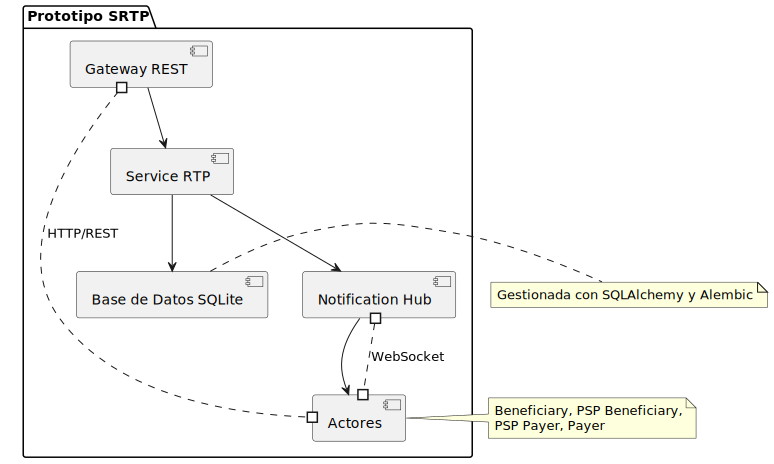
\includegraphics[width=.85\textwidth]{Imagenes/DiagComp.pdf}
  \caption{Arquitectura lógica y flujo de dependencias del prototipo.}
  \label{fig:componentes}
\end{figure}

% Descripción de los componentes principales
\subsection{Componentes principales}
\label{subsec:componentes_principales}
El sistema se estructura en tres componentes principales:
\begin{itemize}
  \item \textbf{Gateway REST}: Actúa como punto de entrada para las solicitudes HTTP, gestionando la validación inicial de las peticiones y enrutándolas al componente adecuado. Este componente asegura que las solicitudes cumplan con los formatos esperados antes de procesarlas.
  \item \textbf{Service RTP}: Encapsula la lógica de negocio del esquema SRTP, incluyendo la creación, validación, enrutamiento y decisión de solicitudes de pago. Interactúa con la base de datos para almacenar y recuperar información.
  \item \textbf{Notification Hub}: Mantiene canales WebSocket abiertos con los cuatro actores del modelo de cuatro esquinas (Beneficiary, PSP Beneficiary, PSP Payer y Payer), enviando notificaciones en tiempo real sobre eventos como la creación o decisión de una solicitud RTP.
\end{itemize}

%----------------------------------------------
% 3.6.2 – Flujo de interacción lógico
%----------------------------------------------
\subsection{Flujo de interacción lógico}
\label{subsec:flujo_interaccion}

El ciclo \textbf{SRTP} se articula en los cuatro pasos lógicos que se detallan a continuación:

\begin{enumerate}[label=\arabic*.]
  \item \textbf{Recepción} – El \emph{Gateway} recibe la petición
        \verb|POST /rtp| y la delega al \emph{Service RTP}.
  \item \textbf{Procesamiento} – El \emph{Service RTP} aplica la lógica de negocio
        y actualiza el estado
        \mbox{\texttt{created} $\rightarrow$ \texttt{validated} $\rightarrow$ \texttt{routed} …}.
  \item \textbf{Publicación} – Tras cada transición de estado válida,
        el servicio emite un evento de dominio.
  \item \textbf{Notificación} – El \emph{Notification Hub} reenvía dicho evento,
        vía WebSocket, a las salas correspondientes
        (\emph{psp\_beneficiary}, \emph{psp\_payer}, \emph{payer} o \emph{beneficiary}).
\end{enumerate}

Con este patrón se obtienen las siguientes ventajas:

\begin{itemize}
  \item Los \emph{clientes} no interrogan al servidor; reciben notificaciones \emph{push}.
  \item La \emph{consistencia} del estado queda centralizada en el \emph{Service RTP}.
  \item El sistema puede escalar horizontalmente añadiendo réplicas del servicio
        sin romper el contrato público.
\end{itemize}



\section{Emulación del flujo RTP}
\label{subsec:emulacion_flujo_rtp}

% Inclusión de la figura de la máquina de estados
\begin{figure}[htbp]
  \centering
  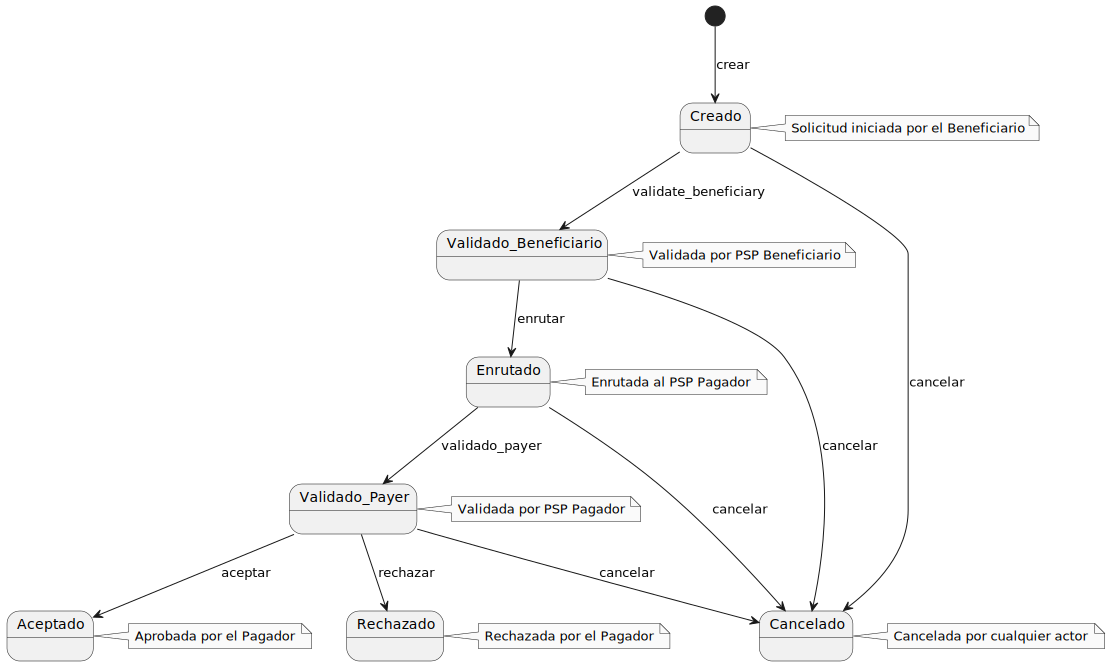
\includegraphics[width=.85\textwidth]{Imagenes/DiagEstado.pdf}
  \caption{Máquina de estados del objeto RTP.}
  \label{fig:state_machine_rtp}
\end{figure}

El objetivo de este apartado es describir cómo el prototipo recrea, de extremo a extremo, el ciclo de vida de una solicitud RTP dentro del bloque \textbf{Service RTP}, único responsable de aplicar la lógica de negocio y salvaguardar la coherencia del estado global. A diferencia de otros componentes, este servicio actúa como \emph{single source of truth}: valida, persiste, publica eventos de dominio y rechaza cualquier transición inválida.

\subsection{Máquina de estados del objeto RTP}
\label{subsec:rtp_state_machine}

La Figura~\ref{fig:state_machine_rtp} sintetiza el recorrido que puede seguir una solicitud:  
\textbf{Creado $\rightarrow$ Validado Beneficiario $\rightarrow$ Enrutado $\rightarrow$ Validado Payer $\rightarrow$ (Aceptado $|$ Rechazado $|$ Cancelado)}.  
Cada arista representa una operación expuesta por la API (por ejemplo, \texttt{create}, \texttt{validate\_beneficiary}, \texttt{route}, \texttt{validate\_payer}, \texttt{accept}, \texttt{reject}, \texttt{cancel}) y sólo puede ejecutarse si el objeto se encuentra en el estado de origen indicado.

\subsection{Transiciones y reglas de negocio}

\begin{description}
  \item[\textbf{Creación} (\texttt{create})]  
        El \emph{Beneficiary} emite un \texttt{POST /rtp}. \textbf{Service RTP} valida sintaxis y semántica (IBAN, ISO 4217, etc.), calcula un hash SHA-256 para evitar duplicados y persiste el registro como \textsc{CREADO}.
  \item[\textbf{Validación del PSP Beneficiary} (\texttt{validate\_beneficiary})]  
        El PSP del beneficiario comprueba el cumplimiento de las reglas SRTP (formato, AML/KYC básico). Si falla, genera un \texttt{reject} inmediato con motivo normalizado.
  \item[\textbf{Enrutado} (\texttt{route})]  
        Una vez validada, la solicitud se envía al PSP \emph{Payer}. El estado avanza a \textsc{ENRUTADO} y se incorpora un \texttt{timestamp} a la traza.
  \item[\textbf{Validación del PSP Payer} (\texttt{validate\_payer})]  
        El PSP del pagador confirma que el cliente puede recibir la solicitud. La aprobación conduce a \textsc{VALIDADO\_PAYER}; de lo contrario, devuelve \texttt{reject}.
  \item[\textbf{Decisión del Payer} (\texttt{accept} / \texttt{reject})]  
        El pagador dispone de un máximo de diez segundos para responder. La aceptación transita a \textsc{ACEPTADO}; la denegación, a \textsc{RECHAZADO}.
  \item[\textbf{Cancelación} (\texttt{cancel})]  
        Cualquiera de los cuatro actores puede solicitar la anulación antes de la decisión final, llevando el flujo a \textsc{CANCELADO}.
\end{description}

Todas las reglas están encapsuladas en métodos de dominio homogéneos en firma y manejo de errores, favoreciendo la mantenibilidad y la trazabilidad entre diseño y código.

\subsection{Condiciones excepcionales y \emph{timeouts}}

Si el pagador no responde antes de la \textbf{fecha/hora de expiración} definida en la solicitud, el sistema ejecuta una transición automática a \textsc{CANCELADO}. Del mismo modo, cualquier error técnico de un PSP desemboca en un \texttt{reject}, manteniendo la consistencia global sin intervención manual.
%
%\subsection{Resumen}
%
%El modelo de estados implementado consagra tres principios:
%
%\begin{enumerate}
%  \item \textbf{Centralización}: toda la lógica reside en \textbf{Service RTP}, evitando duplicidades y condiciones de carrera.
%  \item \textbf{Observabilidad}: cada evento se persiste, firma y publica, facilitando auditoría y \emph{monitoring}.
%  \item \textbf{Extensibilidad}: la adición de nuevos estados o transiciones (p.\,ej.\ \emph{refund}) sólo requiere ampliar la máquina y los servicios asociados, sin impactar capas externas.
%\end{enumerate}
%
%
%Con ello, la emulación demuestra que el ciclo SRTP puede implementarse de forma robusta y trazable aprovechando patrones de \emph{domain-driven design} y mensajería asíncrona, sentando las bases para una futura conexión con infraestructuras de pago reales.
